% Chapter nl: the note of October 20, 2026, assembled for the compendium -- do not edit by hand
\chapter{Nonlinear inverse bremsstrahlung and the efficiency of gas lasers}\label{nl:chapter}
\notedate{October 20, 2026}
\begingroup
\noindent\emph{Inverse bremsstrahlung absorption is nonlinear: a strong enough field
reshapes the electron distribution that absorbs it, as Langdon showed, as Milder et
al.\ observed directly and as Turnbull et al.\ have now measured in absorption
\cite{nl:Langdon1980,nl:Milder2021,nl:Turnbull2023,nl:Turnbull2024}. This note asks whether that
nonlinearity can be used to make gas lasers more efficient. It locates the lasers
and the available sources against the thresholds of the three nonlinearities, builds
a kinetic equation for Langdon's and the gas's nonlinearity (the field, electron--atom
and electron--ion collisions, and the electron--electron collisions that oppose the
field, in the classical small-angle form of the collision integral whose quantum form
is derived in \cite{nl:QBE}), checks it against Langdon's absorption factor, and applies
it to the KrF laser gas, with growing and with beam-sustained electrons, and to the
target that excimer drivers illuminate. Silin's regime is reached nowhere here. Every
number computed here is checked numerically, as Appendix~\ref{nl:app:checks}
describes. The results are in silico.}

\medskip
\noindent SI units are used, with electron energies $\epsilon$ and
temperatures $T$ in eV. The isotropic electron distribution $F(\epsilon)$ is
normalized as $\int_0^\infty\epsilon^{1/2}F\,\dd\epsilon=1$, $\gamma=(2e/m)^{1/2}$,
$v=\gamma\epsilon^{1/2}$, and $1~\mathrm{Td}=10^{-21}$~V\,m$^2$. A field
$E_0\cos\omega t$ has the rms value $E=E_0/\sqrt2$, the quiver amplitude
$v_0=eE_0/m\omega$ and, for linear polarization, the intensity
$I=c\epsilon_0E_0^2/2$. Two fills of the KrF laser gas are used: the Ne fill,
Ne/Kr/F$_2$ $=0.948/0.05/0.002$ at 2~atm, and the Ar
fill, Ar/Kr/F$_2$ $=0.597/0.40/0.003$ at 1~atm, both at 300~K, with the LXCat
cross sections BSR for neon, Biagi-v7.1 for krypton,
IST-Lisbon for argon and SIGLO for F$_2$ \cite{nl:LXCat}. The ions (cations and F$^-$)
are taken to number $1.15\,n_e$ at every $n_e$, the mean over the pump window that a
kinetic model of an electron-beam-pumped laser gives for Kr/F$_2$ at 665~Torr with
2.8~Torr of F$_2$, taken for both fills. A revised form of that model gives 1.35, and
with it krypton's share at beam-on density moves by at most 0.02 points.


\section{The question and the answer}
\label{nl:sec:answer}

{\noindent}(1) A gas laser converts the energy of its electrons into
excitation. The efficiency of that step depends on the shape of the electron
distribution, because the excitation thresholds sit in its tail. Inverse
bremsstrahlung (IB) is the way a field of frequency $\omega$ heats electrons,
and its nonlinearity is that the heating reshapes the distribution. The
question is whether a gas laser can be run in the nonlinear regime, by its own
field or by an auxiliary one, so that the reshaped distribution puts more of
the electrons' energy where the laser wants it.

{\noindent}(2) The answer has four parts.
\begin{itemize}
\item The lasing field of an excimer laser is linear. At a few saturation
  intensities (10~MW\,cm$^{-2}$ for KrF, 30 for ArF) its intensity is $10^{3.8}$ to
  $10^{4.2}$ times below the intensity at which IB alone would supply the electrons'
  energy budget at $T_e=1.5$~eV (at least $1.4\times10^3$ times for $T_e$ from 1.08
  to 2.04~eV), and further still below Langdon's and Silin's thresholds
  (Sec.~\ref{nl:sec:regime}). Of the lasers examined, the CO$_2$ laser is the
  exception: by an order-of-magnitude estimate its own field supplies about a tenth of
  its discharge electrons' budget at 100~MW\,cm$^{-2}$.
\item An auxiliary field (microwave to far infrared) reaches only the
  nonlinearity of a weakly ionized gas, in which the field sets the electron
  temperature. It does so long before Langdon's flattening or Silin's saturation,
  which need tens and hundreds of times more intensity (33 to 80 and 380 to 920 times
  at the temperatures of Table~\ref{nl:tab:regime}).
\item In that regime the frequency is a real lever on the distribution while
  electron--electron collisions are rare. A field far above the collision frequency
  roughly doubles krypton's share of the absorbed power at low power ($\times2.0$ to
  $\times2.1$ in the Ne fill at the power of 2~Td and $\times2.1$ to $\times2.4$ in the
  Ar fill at 6~Td, with growing or with beam-sustained electrons at a fixed electron
  density), and multiplies it
  by 12 to 32 in the Ar fill at 3~Td, where the DC share is only 1 to 5~\%. Those
  collisions remove most of the lever at the densities of a pumped laser. Where the
  lever is large they do not spoil the high-frequency distribution: they pull both
  distributions towards the Maxwellian, and the DC one catches up. The advantage
  halves at a generalized Langdon parameter $\alpha_g=0.41$ to 0.55. At the
  beam-on density of a pumped laser, $2.72\times10^{21}$~m$^{-3}$, with the growth model or with
  beam-sustained electrons that recombine as Kr$_2^+$, it is 2 to 7~\% where the field's
  power exceeds the beam's own and 10 to 14~\% at a fixed beam current where the beam's is
  larger (up to 27~\% at fixed $n_e$). Without recombination it is 1 to 18~\%, and 3 to
  7~\% at a fixed beam current. With one electron per ion pair the beam-sustained model
  holds that density only with 13 times the beam power that gives it in a full kinetic
  model of the laser, and at the five times lower
  density it holds with that power the advantage is up to $\times1.24$ at a fixed beam
  current and $\times1.355$ at fixed $n_e$ (Sec.~\ref{nl:sec:source}). The krypton
  share of a
  self-sustained discharge differs from its DC value by at most 1.5 percentage points
  in the Ne fill, and falls by up to ten points at high frequency in the Ar fill
  (Secs.~\ref{nl:sec:share} and~\ref{nl:sec:selfsus}).
\item At the target the nonlinearity favours the short wavelengths of the gas
  lasers. At the quarter-critical conditions that NRL computed for 351, 248 and
  193~nm, the Langdon factor of a homogeneous plasma is 0.94, 0.96 and 0.98 with the
  velocity-dependent logarithm. That factor alone raises the local absorption rate of
  KrF and ArF light by 2.3 and 3.8~\% over 351~nm, on top of the much larger linear
  gain of the short wavelengths. Speckle and nonlocal transport, left out here, may
  change it (Sec.~\ref{nl:sec:ife}).
\end{itemize}

{\noindent}(3) The nonlinearity of IB is therefore not, by itself, a lever on
the efficiency of a gas laser. What the computation does show is nearly
frequency-blind and favourable. Field pumping of the beam-ionized Ne fill at beam-on
density puts 0.30 to 0.35 of the absorbed energy into KrF$^*$ where its power exceeds
the beam's own, counted at the photon energy, depending on the power and on the
electron-source model. The e-beam itself reaches 0.20 in the same accounting once its
sub-excitation electrons are credited, so field pumping forms 1.5 to 1.8 times as much
there, and the frequency moves that by $-4$ to $+6$~\% (Sec.~\ref{nl:sec:wallplug}). The accounting leaves out electron collisions
with Kr$^*$ and KrF$^*$, which compete with the formation at beam-on density. Whether
field pumping pays is a question of source efficiency, stability and chemistry, which
this note does not address. The most useful
application of the nonlinear absorption is an instrument: a THz pulse that sets
$T_e$ on demand and a transmission that reads it back.

\section{Three nonlinearities of inverse bremsstrahlung}
\label{nl:sec:three}

{\noindent}(1) \emph{Langdon's nonlinearity: the distribution flattens.} In a
fully ionized plasma with $\omega\gg\nu_{ei}$ the field heats electrons through
their collisions with ions with the velocity-space diffusion coefficient
$(v_0^2/6)\nu_{ei}(v)$ \cite{nl:Langdon1980}, and $\nu_{ei}\propto v^{-3}$ heats the slow
electrons most. Electron--electron collisions restore the Maxwellian. Their
competition is measured by Langdon's parameter
\begin{equation}
\alpha_L=\frac{Z_{\rm eff}v_0^2}{v_t^2},\qquad v_t^2=\frac{eT}{m},\qquad
Z_{\rm eff}=\frac{\langle Z^2\rangle}{\langle Z\rangle},
\label{nl:eq:alphaL}
\end{equation}
As $\alpha_L$ grows the distribution becomes flat-topped, which lowers the absorption
by the factor $f_L$. Langdon found the absorption 12~\% lower at $\alpha_L=0.05$, 67~\%
of its Maxwellian value at 0.5 and 45~\% in the limit \cite{nl:Langdon1980}.
This note takes the onset at $\alpha_L=0.1$, where the self-similar solution of
Sec.~\ref{nl:sec:checks} gives $f_L=0.83$ (Langdon's fit 0.82). Turnbull
et al.\ measured the absorption of a 527~nm probe in gas-jet plasmas and found that it
needs this factor \cite{nl:Turnbull2023}. The path-integrated $f_L$ averaged 0.76 over all
their data, and even over the eight pure-hydrogen shots it averaged 0.81 and fell as
low as 0.74.

{\noindent}(2) \emph{Silin's nonlinearity: the quiver outruns the electron.} When
$v_0\gtrsim v_t$ the collision samples the oscillating relative velocity and the
absorption falls as $(v_t/v_0)^3$ up to a logarithm \cite{nl:Silin1965}.

{\noindent}(3) \emph{The nonlinearity of a weakly ionized gas: the field sets the
temperature.} In a laser gas, $n_e/N$ is $10^{-7}$ to $10^{-4}$ and electrons lose
energy mainly to atoms and molecules. Elastic collisions remove only the fraction
$2m/M$ of the energy per collision, $1.3\times10^{-5}$ (Kr) to $5.4\times10^{-5}$ (Ne),
and the inelastic channels raise the effective fraction $\delta_{\rm eff}$ to
$4\times10^{-4}$ to $8\times10^{-4}$ in the excimer fills (Sec.~\ref{nl:sec:regime}) and to
about $10^{-2}$ in a CO$_2$ laser discharge. A field heats
an electron at the rate $P=\sigma_{\rm abs}I$, where, in the Lorentz two-term
approximation,
\begin{equation}
\sigma_{\rm abs}=\frac{e\,{\rm Re}\,\mu(\omega)}{c\epsilon_0}
\;\xrightarrow{\;\omega\gg\nu\;}\;\frac{e^2}{mc\epsilon_0}\,\frac{\nu_{\rm eff}}{\omega^2},
\label{nl:eq:sigabs}
\end{equation}
$\mu$ being the complex mobility. The field takes over the temperature once $P$
exceeds the collisional loss $P_{\rm loss}(T_e)$ that holds $T_e$, at
\begin{equation}
I_{\rm heat}=\frac{P_{\rm loss}(T_e)}{\sigma_{\rm abs}(\omega)},\qquad
I_L(\alpha_L)=\frac{c\epsilon_0}{2}\Big(\frac{m\omega}{e}\Big)^2\frac{\alpha_L\,eT}{mZ_{\rm eff}},\qquad
I_S=\frac{c\epsilon_0}{2}\Big(\frac{m\omega}{e}\Big)^2\frac{eT}{m},
\label{nl:eq:thresholds}
\end{equation}
the last two being the intensities of a given $\alpha_L$ and of $v_0=v_t$. For
$\omega\gg\nu$, Eqs.~\eqref{nl:eq:sigabs} and \eqref{nl:eq:thresholds} give
\begin{equation}
\frac{I_L}{I_{\rm heat}}=\frac{\alpha_L\,eT\,\nu_{\rm eff}}{2Z_{\rm eff}P_{\rm loss}}
=\frac{\alpha_L}{3Z_{\rm eff}\,\delta_{\rm eff}},\qquad
P_{\rm loss}=\tfrac32\,eT\,\delta_{\rm eff}\,\nu_{\rm eff}.
\label{nl:eq:ratio}
\end{equation}
A gas's electrons thus answer to an intensity $\alpha_L/3Z_{\rm eff}\delta_{\rm eff}$ times
lower than the one that gives a plasma's distribution a given $\alpha_L$, 33 to 80 times
lower for $\alpha_L=0.1$ at the temperatures of Table~\ref{nl:tab:regime}. $I_{\rm heat}$ is
the threshold that Ginzburg and Gurevich called the plasma field: below it a wave
crosses a weakly ionized plasma without changing it appreciably
\cite{nl:GinzburgGurevich1960,nl:Gurevich1978}.
In the gas, the nonlinearity is that the distribution, and with it $\nu_{\rm eff}$ and
the absorption, follows the field. Its shape depends on $\omega$: a DC field heats
each electron in proportion to $1/\nu_m(\epsilon)$, a field with $\omega\gg\nu_m$
in proportion to $\nu_m(\epsilon)$ (Sec.~\ref{nl:sec:kinetic}).

{\noindent}(4) \emph{The generalized Langdon parameter.} In every case the departure
from the Maxwellian is decided by the field's heating against the Maxwellization by
electron--electron collisions, while in a gas the energy dependence of $\nu_m$ and the
inelastic losses also set its form. Define
\begin{equation}
\alpha_g=\frac{P_{\rm abs}}{eT_e\,\nu_{ee}},\qquad
\nu_{ee}=2.91\times10^{-12}\,n_e\,\lnL\,T_e^{-3/2}~{\rm s}^{-1}
\quad(n_e~\text{in m}^{-3},\;T_e~\text{in eV}),
\label{nl:eq:alphag}
\end{equation}
with $P_{\rm abs}$ the absorbed power per electron and $\nu_{ee}$ the electron
collision rate of the NRL formulary \cite{nl:NRL}. For the Maxwellian of a fully ionized plasma
the IB heating is $P=(e^2E^2/m\omega^2)\,\nu_TL$ with
$\nu_T=(4\sqrt{2\pi}/3)\,n_iZ^2e^4/[(4\pi\epsilon_0)^2m^{1/2}(eT)^{3/2}]$
\cite{nl:Atzeni2004}. In practical units
$\nu_T=2.906\times10^{-12}\,n_iZ^2T^{-3/2}$, the coefficient of $\nu_{ee}$, so
\begin{equation}
\alpha_g=\frac{\alpha_L}{2}\,\frac{L}{\lnL},
\label{nl:eq:alphag-alphaL}
\end{equation}
and Langdon's $\alpha_L$ is $2\alpha_g$ when the two logarithms are equal. The
same $\alpha_g$ applies to a gas, where $P_{\rm abs}$ comes mostly from collisions
with atoms.

\section{The kinetic equation}
\label{nl:sec:kinetic}

{\noindent}(1) The isotropic part of the distribution obeys, in the two-term
approximation and per electron,
\begin{equation}
\epsilon^{1/2}\frac{\partial F}{\partial t}=-\frac{\partial G}{\partial\epsilon}+S[F],\qquad
G=G_{\rm field}+G_{\rm el}+G_{ee},
\label{nl:eq:kinetic}
\end{equation}
with $S$ the inelastic collisions (and the source or growth term of item~(6)). The
field flux is $G_{\rm field}=-D_{\rm field}F'$ with
\begin{equation}
D_{\rm field}=\frac{\gamma^2}{3}\,E^2\epsilon^{3/2}\,\frac{\nu}{\nu^2+\omega^2},\qquad
\nu=\nu_a+\nu_c,
\label{nl:eq:Dfield}
\end{equation}
where $\nu_a=N\gamma\epsilon^{1/2}\sigma_m$ is the momentum-transfer frequency on
atoms and $\nu_c$ that on ions. At $\omega=0$ this is the DC term of Hagelaar and
Pitchford \cite{nl:HP2005}, $D=(\gamma/3)(E/N)^2\epsilon N/\sigma_m$, and for
$\omega\gg\nu$ it is $(\gamma^2/3)(E/\omega)^2\epsilon^{3/2}\nu$, which is Langdon's
operator with the velocity-space diffusion coefficient $(v_0^2/6)\nu$
\cite{nl:Langdon1980}. The two-term expansion needs a small anisotropy, so it cannot describe
Silin's regime. At every scan point of Secs.~\ref{nl:sec:share} and~\ref{nl:sec:selfsus}
the electrons' oscillation velocity $eE_0/m(\omega^2+\nu_m^2)^{1/2}$, with the
Maxwellian $\langle\nu_m\rangle$ on atoms, is at most $0.13\,v_t$. The elastic flux on atoms is
$G_{\rm el}=-\gamma\epsilon^2N\sigma_\epsilon(F+T_gF')$ with
$\sigma_\epsilon=\sum_jx_j(2m/M_j)\sigma_{m,j}$.

{\noindent}(2) \emph{Ions.} A singly charged ion has the Coulomb
momentum-transfer cross section
\begin{equation}
\sigma_c(\epsilon)=\pi\Big(\frac{e}{4\pi\epsilon_0\,\epsilon}\Big)^2L(\epsilon),\qquad
L=\tfrac12\ln\!\Big[1+\Big(\frac{b_{\max}}{b_{\min}}\Big)^2\Big],
\label{nl:eq:sigc}
\end{equation}
with $b_{\max}=v/(\omega^2+\omega_p^2)^{1/2}$ and $b_{\min}$ the larger of
$e^2/4\pi\epsilon_0mv^2$ and $\hbar/2mv$. For $\omega\gg\omega_p$, $b_{\max}$ is the IB
cutoff $v/\omega$, set by the laser frequency rather than the plasma frequency as
Turnbull et al.\ found the absorption to need \cite{nl:Turnbull2023}. Below $\omega_p$ it
becomes the screening length $v/\omega_p$. Then
$\nu_c=\pi n_iZ^2\gamma(e/4\pi\epsilon_0)^2L\,\epsilon^{-3/2}$, and for
$\omega\gg\nu_c$ Eq.~\eqref{nl:eq:Dfield} becomes, with
$E^2/\omega^2=(v_0^2/v_t^2)\,T/\gamma^2$ and $n_iZ=n_e$,
\begin{equation}
D_{\rm IB}=\frac{\pi\gamma^3}{3}\,n_iZ^2\Big(\frac{e}{4\pi\epsilon_0}\Big)^2L\,\frac{E^2}{\omega^2}
=\frac{\pi\gamma}{3}\,\alpha_L\,T\,n_e\Big(\frac{e}{4\pi\epsilon_0}\Big)^2L.
\label{nl:eq:DIB}
\end{equation}
For a constant logarithm $D_{\rm IB}$ does not depend on $\epsilon$: in energy,
Langdon's operator is pure diffusion with a constant coefficient. The absorbed
power is $P=\int D_{\rm IB}(-F')\,\dd\epsilon=D_{\rm IB}F(0)$, proportional to the
number of slow electrons, so $f_L=F(0)/F_M(0)$ at equal $T$, where $F_M$ is the
Maxwellian.

{\noindent}(3) \emph{Langdon's $v^5$ distribution, exactly.} With heating alone the
distribution obeys $\epsilon^{1/2}\partial_tF=D_{\rm IB}\partial_\epsilon^2F$. Try
$F=A(t)\exp[-\epsilon^{5/2}/b(t)]$. Then
$\epsilon^{1/2}\partial_tF=\epsilon^{1/2}F(\dot A/A+\epsilon^{5/2}\dot b/b^2)$ and
$\partial_\epsilon^2F=F[(25/4)\epsilon^3/b^2-(15/4)\epsilon^{1/2}/b]$. The powers
$\epsilon^{1/2}$ and $\epsilon^3$ match separately when
\begin{equation}
\frac{\dd b}{\dd t}=\frac{25}{4}\,D_{\rm IB},\qquad \frac{\dd\ln A}{\dd t}=-\frac{15}{4}\frac{D_{\rm IB}}{b}.
\label{nl:eq:v5}
\end{equation}
The distribution keeps the shape $\exp(-v^5)$ while it heats, Langdon's limit for
$\alpha_L\to\infty$, and its absorption factor, that of the super-Gaussian
$\exp[-(v/v_m)^M]$ with $M=5$ at the same density and energy, is
$F(0)/F_M(0)=M(\pi/2)^{1/2}\Gamma(5/M)^{3/2}/[3^{3/2}\Gamma(3/M)^{5/2}]=0.4456$.

{\noindent}(4) \emph{Electron--electron collisions.} The isotropic Rosenbluth
operator \cite{nl:Rosenbluth1957} is the classical small-angle (Landau) form of the
electron--electron collision integral, whose quantum form is derived in \cite{nl:QBE}.
In energy it reads (Appendix~\ref{nl:app:ee})
\begin{equation}
G_{ee}=-2a\,n_e\int_0^\infty\min(\epsilon,\epsilon')^{3/2}\big[F(\epsilon')F'(\epsilon)-F(\epsilon)F'(\epsilon')\big]\,\dd\epsilon',\qquad
a=\frac{e^2\gamma\lnL}{24\pi\epsilon_0^2},
\label{nl:eq:ee-landau}
\end{equation}
which is the form $-a\,n_e[3A_1F+2(A_2+\epsilon^{3/2}A_3)F']$ of Hagelaar and
Pitchford \cite{nl:HP2005}, $A_1=\int_0^\epsilon u^{1/2}F$, $A_2=\int_0^\epsilon u^{3/2}F$,
$A_3=\int_\epsilon^\infty F$. The kernel is symmetric and the bracket
antisymmetric in $(\epsilon,\epsilon')$, so
\begin{equation}
\int_0^\infty G_{ee}\,\dd\epsilon=0,
\label{nl:eq:ee-energy}
\end{equation}
which, since $\int\epsilon\,\partial_\epsilon G\,\dd\epsilon=-\int G\,\dd\epsilon$,
is the conservation of energy. Any $F\propto e^{-\epsilon/T}$ makes the bracket
vanish. Far above the bulk, $\min=\epsilon'$, the friction is
$2an_e\int\epsilon'^{3/2}F'\,\dd\epsilon'=-3an_e$ and the diffusion is constant,
so a fast electron loses energy at
\begin{equation}
\frac{\dd(e\epsilon)}{\dd t}=-\frac{3a\,n_e\,e}{\epsilon^{1/2}}
=-\frac{e^4\lnL\,n_e}{4\pi\epsilon_0^2\,m\,v},
\label{nl:eq:spitzer}
\end{equation}
the classical slowing-down rate of a fast electron by the field electrons,
$7.7\times10^{-12}\,n_e\lnL\,\epsilon^{-3/2}$~s$^{-1}$ in the units of
Eq.~\eqref{nl:eq:alphag} \cite{nl:NRL}. Discretized on the cell faces with face averages and
differences of $F$, Eq.~\eqref{nl:eq:ee-energy} holds to round-off and a sampled
Maxwellian is an exact zero for every grid step.

{\noindent}(5) \emph{The heated plasma at fixed $\alpha_L$.} For a fully ionized
plasma heated by IB, write $x=\epsilon/T$ and $F=T^{-3/2}\Phi(x)$ with $T$ two
thirds of the mean energy. When the shape is stationary while $T$ rises, the flux
in the frame that moves with $T$ vanishes everywhere. Dividing by $2an_eT^{-3/2}$,
\begin{equation}
-\beta\,g(x)\Phi'-\big[\Phi'P(x)-\Phi\,Q(x)\big]=\lambda\,x^{3/2}\Phi,\qquad
\beta=\frac{\alpha_LL}{4\lnL},
\label{nl:eq:selfsim}
\end{equation}
with $P=\int\min(x,x')^{3/2}\Phi(x')\,\dd x'$, $Q=\int\min(x,x')^{3/2}\Phi'(x')\,\dd x'$,
$g=L(xT)/L$ for a velocity-dependent logarithm (otherwise 1), and $\lambda$ the
heating rate $\dot T/T$ in e-e units. The ratio $\beta$ follows from
Eq.~\eqref{nl:eq:DIB} and $2an_e=(4\pi/3)\gamma\lnL\,n_e(e/4\pi\epsilon_0)^2$.
Integrating Eq.~\eqref{nl:eq:selfsim} over $x$, the e-e term drops out by
Eq.~\eqref{nl:eq:ee-energy} and $\int x^{3/2}\Phi=3/2$ gives
$\lambda=(2/3)\beta\int g(-\Phi')\,\dd x$. For $\beta\to\infty$,
Eq.~\eqref{nl:eq:selfsim} gives $\Phi\propto\exp(-cx^{5/2})$, the distribution of
Eq.~\eqref{nl:eq:v5}. For $\beta\to0$ it gives the Maxwellian. By
Eq.~\eqref{nl:eq:alphag-alphaL}, $\beta=\alpha_g/2$ for the Maxwellian.

{\noindent}(6) \emph{Method.} \label{nl:sec:method}
Equation~\eqref{nl:eq:kinetic} is solved on an energy grid with the two-term
discretization of Hagelaar and Pitchford \cite{nl:HP2005}, extended by
Eqs.~\eqref{nl:eq:sigc} and \eqref{nl:eq:ee-landau}. Three choices matter, and the first
was forced by checks of Appendix~\ref{nl:app:checks}.
\begin{itemize}
\item A scheme whose inelastic gains are not exactly number-conserving, and whose
  LU solve replaces the top row by the normalization, satisfies the rows of the tail
  only to the accuracy of the largest $F$. Against an elimination that satisfies
  every row to round-off, such an LU solution
  is off by 2~\% where $F/F_{\max}$ is $10^{-6}$ to $10^{-3}$ and by order one below.
  The solver therefore distributes each source cell's inelastic loss over its
  landing cells (number-conserving to round-off) and solves by Gaussian
  elimination from the top in ratio form, $c_i=F_i/F_{i-1}$, which satisfies
  every row but the lowest. That row is then exactly the particle balance, and
  the growth frequency is found as the root of it. Krypton's share of the power
  changes by $3\times10^{-5}$ between the two schemes.
\item The e-e coefficients are lagged and iterated with Anderson mixing
  \cite{nl:WalkerNi2011} of $\ln F$, so that the tail converges in relative terms.
\item A beam-sustained mode replaces the growth term by electrons injected with
  the sub-excitation spectrum of the beam's secondary electrons that a kinetic
  model of the laser uses (linear on
  $0$ to 9.915~eV, mean 4.506~eV), lost by attachment and by recombination with a cross
  section $\propto1/\epsilon$ (Sec.~\ref{nl:sec:source}).
\end{itemize}

\section{Checks of the kinetic model}
\label{nl:sec:checks}

{\noindent}(1) \emph{Langdon.} Table~\ref{nl:tab:langdon} and
Fig.~\ref{nl:fig:langdon} compare the solutions of Eq.~\eqref{nl:eq:selfsim} with equal
logarithms ($\beta=\alpha_L/4$) to Langdon's fit
$f_L=1-0.553/[1+(0.27/\alpha_L)^{0.75}]$, which he gives as good to $\pm0.005$
\cite{nl:Langdon1980} and Turnbull et al.\ use \cite{nl:Turnbull2023}. They agree within
1.8~\% from $\alpha_L=0.01$ to 100, the largest difference being at $\alpha_L=0.5$. The kinetic solution is therefore
the problem Langdon solved. The fitted super-Gaussian exponent depends on the
fit, because the distribution is not exactly super-Gaussian. Matte's
$m(\alpha_L)=2+3/(1+1.66\alpha_L^{-0.724})$ \cite{nl:Matte1988,nl:Turnbull2024} lies
between the exponents of two fits for $\alpha_L\le5$ and within 0.09 of the
three-parameter fit above. The energy relation of item~(5) of
Sec.~\ref{nl:sec:kinetic} holds to $3\times10^{-6}$, and $\beta\to\infty$ reproduces
the $v^5$ distribution's factor 0.4456 to $4\times10^{-6}$.

\begin{table}[h]
\centering
\caption{The heated plasma at fixed $\alpha_L$, Eq.~\eqref{nl:eq:selfsim} with
$\beta=\alpha_L/4$, against Langdon's absorption fit and Matte's exponent.
$m$ is fitted in two ways: to $\ln\ln(\Phi(0)/\Phi)$ against $\ln x$ on
$0.1<x<3$, and with three free parameters on $x<3$.}
\label{nl:tab:langdon}
\begin{tabular}{rcccccc}
\toprule
$\alpha_L$ & $f_L$ & Langdon's fit & ratio & $m$, $\ln\ln$ & $m$, three-parameter & Matte's $m$\\
\midrule
\tabinput{chapters/nl/tab_langdon.tex}
\bottomrule
\end{tabular}
\end{table}

\begin{figure}[h]
\centering
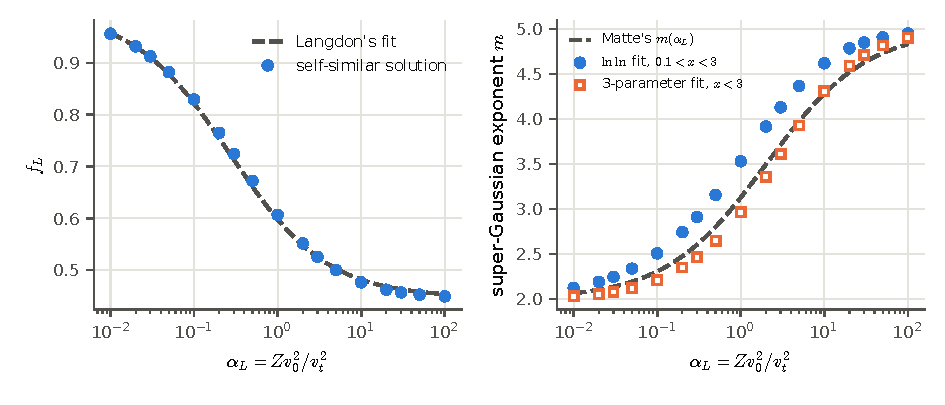
\includegraphics[width=\textwidth]{chapters/nl/fig_langdon.pdf}
\caption{Left: the absorption factor of the heated plasma against Langdon's
fit. Right: fitted super-Gaussian exponents against Matte's.}
\label{nl:fig:langdon}
\end{figure}

{\noindent}(2) \emph{The gas.} With $n_e=0$, no ions and the discretization of
the first scheme of Sec.~\ref{nl:sec:method}, the solver reproduces an independent
two-term solver to $7\times10^{-11}$. A
constant cross section in a DC field gives the Druyvesteyn distribution
\cite{nl:Druyvesteyn1940} to $1.2\times10^{-7}$ in $\ln F$, a field with $\omega\gg\nu$ and
elastic losses the Maxwellian of Margenau \cite{nl:Margenau1946}, with or without
e-e collisions. The e-e flux conserves energy to $1.4\times10^{-17}$, its drift on a fast
electron is Spitzer's Eq.~\eqref{nl:eq:spitzer} to $2\times10^{-5}$, and two mixed
Maxwellians relax to one. The Coulomb heating of a 3~eV Maxwellian is
$(e^2E^2/m\omega^2)\nu_TL$ to $9\times10^{-5}$, once the half cell next to $\epsilon=0$
is accounted for. In a DC field e-e collisions turn the Druyvesteyn
distribution, whose $(2/3)\langle\epsilon\rangle/T_{\rm slope}$ is 1.50 with $T_{\rm slope}$
fitted to $\ln F$ on $0.1\langle\epsilon\rangle<\epsilon<4\langle\epsilon\rangle$, into a
Maxwellian: the ratio is 1.0005 at $n_e/N=10^{-2}$.

\section{Where gas lasers sit}
\label{nl:sec:regime}

{\noindent}(1) Table~\ref{nl:tab:regime} evaluates Eq.~\eqref{nl:eq:thresholds} for the
fields of three lasers and for auxiliary sources heating the Ne fill, with
Maxwellian electrons, the losses of the LXCat sets, and the ions of Eq.~\eqref{nl:eq:sigc}.
Every beam-on row has $T_e=1.5$~eV, between the temperature of a Maxwellian power
balance at beam-on density, 1.08~eV, and that of the beam-sustained electrons of
Sec.~\ref{nl:sec:share} at
beam-on density, 1.88 (Ar fill) and 2.04~eV (Ne fill), and $n_e=2.72\times10^{21}$~m$^{-3}$. The
afterglow rows have 0.63~eV and $10^{20}$~m$^{-3}$. The ArF fill is
Electra's, Ar/F$_2$ $=0.997/0.003$ at 0.82~atm \cite{nl:Obenschain2020}. The CO$_2$ row
uses a CO$_2$:N$_2$:He $=1:1:8$ mixture at 1~atm, $T_e=1$~eV and $n_e=10^{19}$~m$^{-3}$
with the IST-Lisbon cross sections \cite{nl:LXCat}, and singly charged cations only ($Z_{\rm eff}=1$).
Langdon's and Silin's intensities are left out where $\nu_m>\omega$, where the
electrons do not quiver freely. Figure~\ref{nl:fig:regime} shows the thresholds against
frequency.

\begin{table}[h]
\centering
\caption{Thresholds of the three nonlinearities, Eq.~\eqref{nl:eq:thresholds}, in
W\,cm$^{-2}$. $u=\hbar\omega/eT_e$; $\nu_m/\omega$ with the Maxwellian
$\langle\nu_m\rangle$; $P_{\rm loss}$ in eV\,s$^{-1}$ per electron; Langdon at
$\alpha_L=0.1$ with $Z_{\rm eff}=1.15$ (1 for the CO$_2$ discharge); Langdon and Silin
left out where $\nu_m>\omega$.}
\label{nl:tab:regime}
\footnotesize
\setlength{\tabcolsep}{3.5pt}
\begin{tabular}{lcccccccc}
\toprule
field, gas & $T_e$ & $n_e$ (m$^{-3}$) & $u$ & $\nu_m/\omega$ & $P_{\rm loss}$ & $I_{\rm heat}$ & $I_L$ & $I_S$\\
\midrule
\tabinput{chapters/nl/tab_regime.tex}
\bottomrule
\end{tabular}
\end{table}

\begin{figure}[h]
\centering
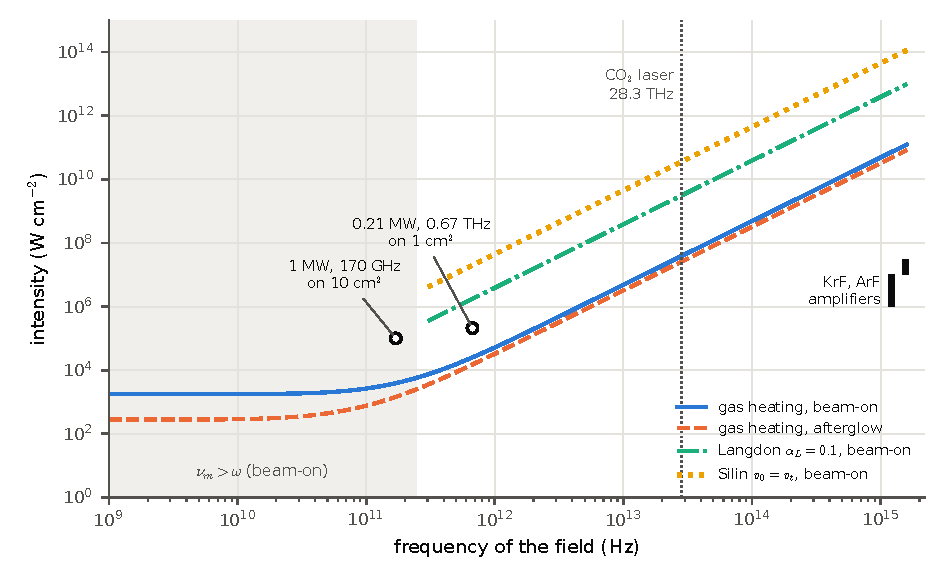
\includegraphics[width=0.9\textwidth]{chapters/nl/fig_regime.pdf}
\caption{The three thresholds against frequency in the Ne fill: gas heating
($I_{\rm heat}$) beam-on ($T_e=1.5$~eV, $n_e=2.72\times10^{21}$~m$^{-3}$) and in the
afterglow ($0.63$~eV, $10^{20}$~m$^{-3}$), Langdon at $\alpha_L=0.1$ and Silin,
both beam-on and drawn only where $\nu_m<\omega$. Bars: KrF amplifiers at 1 to 10 and
ArF amplifiers at 10 to 30~MW\,cm$^{-2}$ (Sec.~\ref{nl:sec:regime}); dotted line: the
CO$_2$-laser frequency 28.3~THz; circles: a 1~MW gyrotron at 170~GHz
\cite{nl:Sakamoto2007} and a 0.21~MW, 0.67~THz gyrotron \cite{nl:Glyavin2012},
each on an assumed spot.}
\label{nl:fig:regime}
\end{figure}

{\noindent}(2) \emph{The lasers' own fields.} An amplifier extracts at a few
saturation intensities. For KrF, $I_{\rm sat}=h\nu(A+Q)/\sigma$ is 1.0 and
1.2~MW\,cm$^{-2}$ in the two fills, with the cross section $2.6\times10^{-16}$~cm$^2$ and
radiative rate of Kannari et al.\ \cite{nl:Kannari1985} and the quench rates of a KrF
kinetic network at each fill's composition. Electra's ArF amplifier
saturates at 10~MW\,cm$^{-2}$ \cite{nl:Obenschain2020}. At 10~MW\,cm$^{-2}$ the KrF field is
$7.1\times10^3$ times below $I_{\rm heat}$ in the Ne fill and $1.5\times10^4$ times in the
Ar fill, and at 30~MW\,cm$^{-2}$ the ArF field is $5.8\times10^3$ times below it. These
margins depend on $T_e$ through the inelastic losses: for $T_e$ from 1.08 to 2.04~eV they
are $10^{3.2}$ to $10^{5.0}$. They also rest on the classical kernel at
$u=\hbar\omega/eT_e=3.3$ and 4.3, where it is not validated (the quantum absorption
on these atoms, from exact phase shifts of model potentials, is 10 to 28~\% below it at
$u=4.5$, for 300~K electrons at 28.3~THz, and its size for 5.0 and 6.4~eV photons
is not known). The excimer lasers' own fields are linear by every measure. The CO$_2$
laser's field supplies a tenth (0.10) of the energy budget of its discharge electrons at
100~MW\,cm$^{-2}$, and all of it at $I_{\rm heat}=9.6\times10^8$~W\,cm$^{-2}$. That is an
order-of-magnitude estimate. It assumes Maxwellian electrons at 1~eV, which at
$n_e/N=4\times10^{-7}$ nothing Maxwellizes, and discharge electrons present while the
pulse passes, which depends on the timing of the amplifier. Of the lasers examined it
is the one in which the lasing field can reach the gas nonlinearity. Lasing is known to perturb CO$_2$-laser
discharges, the optogalvanic effect, but through the vibrational kinetics of the laser levels
\cite{nl:Tachikawa1990}. No study was found of the field's IB heating of the
discharge electrons as an efficiency or stability term.

{\noindent}(3) \emph{Auxiliary fields.} Heating the Ne fill's electrons takes
$1.4\times10^3$~W\,cm$^{-2}$ at 170~GHz and $1.5\times10^4$~W\,cm$^{-2}$ at 0.67~THz
in the afterglow, and $5.2\times10^4$~W\,cm$^{-2}$ at 1~THz beam-on, within reach of
gyrotron beams \cite{nl:Sakamoto2007,nl:Glyavin2012}. Such a beam heats only its absorption length,
2.5~mm at 170~GHz and 2.6~cm at 0.67~THz in the afterglow and 1.1~mm at 1~THz beam-on.
Where $\nu_m<\omega/2$, Langdon's $\alpha_L=0.1$ needs 62 to 80 times $I_{\rm heat}$ in
the Ne fill beam-on, 33 to 51 times in its afterglow, and 37 and 54 times at the laser
frequencies of the Ar and ArF fills. Silin's $v_0=v_t$ needs a further
$Z_{\rm eff}/\alpha_L=11.5$ times. For $\omega\gg\nu_m$ the ratio is
Eq.~\eqref{nl:eq:ratio}, $\alpha_L/3Z_{\rm eff}\delta_{\rm eff}$, with
$\delta_{\rm eff}=4\times10^{-4}$ to $8\times10^{-4}$. In the excimer fills a field strong enough to matter is in the gas
nonlinearity, and only there. The CO$_2$ discharge, whose vibrational losses make
$\delta_{\rm eff}$ large, has Langdon's intensity only 2.5 times its $I_{\rm heat}$.

\section{Frequency as a lever on the distribution}
\label{nl:sec:share}

{\noindent}(1) Without e-e collisions a field above the collision frequency puts
more of its power into krypton than a DC field of the same absorbed power: at the
lowest power about twice as much in the Ne fill and up to 32 times as much in the Ar
fill, where the DC share is 1.3~\%. This section asks whether e-e collisions erase
that. The mechanism is item~(3) of Sec.~\ref{nl:sec:three}. A DC
field heats each electron in proportion to $1/\nu_m$, so in a gas whose $\nu_m$ rises
with energy it heats the slow electrons most and gives the Druyvesteyn-like
distribution, with a depleted tail. A field with $\omega\gg\nu_m$ heats in
proportion to $\nu_m$, which with elastic losses gives Margenau's Maxwellian
\cite{nl:Margenau1946}. Its tail reaches the 9.9~eV krypton levels. That the energy
dependence of $\nu_m$ decides how DC and microwave distributions differ is known for
discharges in general \cite{nl:Karoulina1988}, high-frequency argon distributions have
been computed from $\omega\ll\nu$ to $\omega\gg\nu$ \cite{nl:FerreiraLoureiro1983}, and e-e
collisions were added for argon discharges \cite{nl:Sa1992,nl:Wang1993}. What is new here is
the KrF laser gas and its formation chain. A scan repeats the comparison
at the absorbed powers per electron of DC fields of 2, 5 and 10~Td in the Ne fill and
3, 6 and 15~Td in the Ar fill, with e-e collisions
and ions at each electron density, and with the temporal-growth model of two-term
solvers: the electrons grow or decay with the shape of $F$. Item~(3) repeats it with
electrons born from the beam. The scan treats the field as given inside the gas. At beam-on density the
plasma frequency is 0.47~THz, so a 0.3~THz wave would not enter the gas there. How a
field reaches the gas is a separate question of coupling.

{\noindent}(2) Table~\ref{nl:tab:share} and Fig.~\ref{nl:fig:share} give the result.
Electron--electron collisions raise krypton's share in the DC field, from 27.5 to
80.1~\% at the power of 2~Td in the Ne fill, as $n_e$ rises from 0 to the beam-on
density $2.72\times10^{21}$~m$^{-3}$. The 28.3~THz field goes from 54.2 to
84.5~\%. Collisions bring both towards the Maxwellian, which is where the high
frequency was already taking the distribution. At the 9.9~eV krypton threshold,
relative to a Maxwellian of the same mean energy, the DC distribution holds 0.556
of the population and the 28.3~THz one 0.742 without e-e collisions, and 0.900 and
0.969 at beam-on density. Over the 30 series of the scan that
ratio moves towards 1 between $n_e=0$ and beam-on density in 29, and stays at 0.94 in
the Ar fill at 6~Td and 3~THz. Where the advantage is large, at 2~Td in the Ne fill
and at 3 and 6~Td in the Ar fill, the 28.3~THz ratio rises and the DC one rises more.
The advantage of the frequency therefore falls from
$\times1.97$ to $\times1.055$. Normalized by its value without e-e collisions,
the advantage falls along nearly one curve of $\alpha_g$ for the three power levels
in Fig.~\ref{nl:fig:share}. It halves at $\alpha_g=0.41$, 0.46 and 0.55, found by root
finding in $n_e$ between the scan's grid points. At beam-on
density $\alpha_g$ is 0.023 to 0.14 for these three levels and the frequency is
worth 2.0 to 5.5~\%. In the Ne fill at the highest power, 10~Td, the high frequency
is worse than DC. The fatter tail excites neon itself (its share rises from 1.9 to
7.2~\%), and krypton's share falls by 3.0 points. In the Ar fill at 15~Td the high
frequency is still 2.9 points better without e-e collisions, and 0.6 points worse at
beam-on density.

\begin{table}[h]
\centering
\caption{Krypton's share of the absorbed power (\%) and the formation efficiency
$\eta_{\rm form}$ of Sec.~\ref{nl:sec:wallplug}, DC against 28.3~THz at the same absorbed
power per electron (that of a DC field of the given $E/N$ without e-e
collisions). $\alpha_g$ of the DC point, Eq.~\eqref{nl:eq:alphag}.}
\label{nl:tab:share}
\setlength{\tabcolsep}{5pt}
\begin{tabular}{lccccccc}
\toprule
fill, power & $n_e$ (m$^{-3}$) & $\alpha_g$ & Kr, DC & Kr, 28.3~THz & ratio & $\eta_{\rm form}$, DC & $\eta_{\rm form}$, 28.3~THz\\
\midrule
\tabinput{chapters/nl/tab_share.tex}
\bottomrule
\end{tabular}
\end{table}

\begin{figure}[h]
\centering
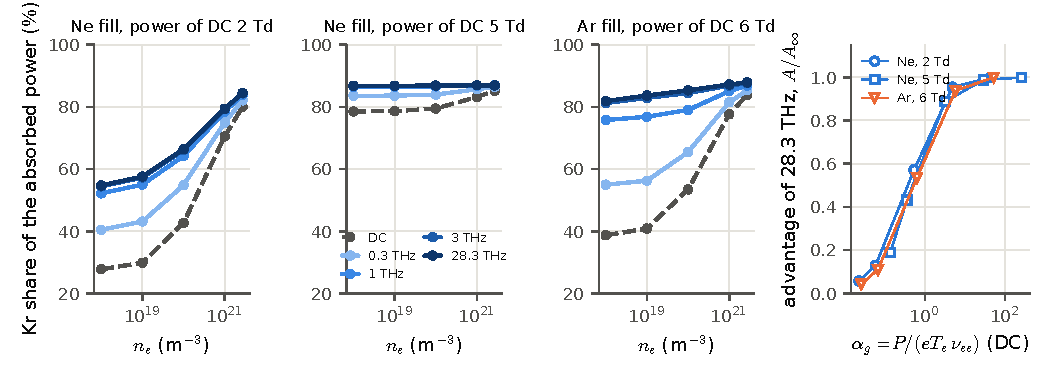
\includegraphics[width=\textwidth]{chapters/nl/fig_share.pdf}
\caption{Krypton's share of the absorbed power against $n_e$, DC (dashed) and
0.3, 1, 3 and 28.3~THz, and (right) the advantage of 28.3~THz over DC,
$A=$ ratio $-1$, normalized by its value without e-e collisions, against
$\alpha_g$. Every point drawn has $P_{\rm field}>1.5\,|P_{\rm growth}|$. The Ar fill at
3~Td is not shown: from $10^{19}$~m$^{-3}$ up its points at 1 to 28.3~THz fall below that.}
\label{nl:fig:share}
\end{figure}

{\noindent}(3) \emph{Beam-sustained electrons.} \label{nl:sec:source}The growth model lets new electrons
appear with the shape of $F$, and at the lowest power its term carries up to 0.66 of
the absorbed power at the points kept, those with $P_{\rm field}>1.5\,|P_{\rm growth}|$.
In an e-beam pumped gas the electrons are born from the beam and lost by attachment and
by recombination. A second scan therefore repeats the comparison at the
absorbed powers of Table~\ref{nl:tab:share} with electrons injected with the beam's
sub-excitation spectrum (item~(6) of Sec.~\ref{nl:sec:kinetic}) and lost by attachment and
by dissociative recombination on $1.075\,n_e$ cations, taken as Kr$_2^+$ with the rate
$2.24\times10^{-7}\,T_e^{-1/2}$~cm$^3$\,s$^{-1}$, built on the dissociative recombination
rates of Kannari et al.\ \cite{nl:Kannari1985}. The loss has a cross
section $\propto1/\epsilon$, which gives that rate for a Maxwellian, so it takes the slow
electrons first. At beam-on density recombination removes electrons 3.1 (Ne fill) and 3.9 (Ar
fill) times faster than attachment, and with the DC field the beam's own injected power
is then 2.4 to 8.3 times the field's, except at 5~Td in the Ne fill (0.425).
Table~\ref{nl:tab:source}
gives the field's marginal share to krypton at fixed $n_e$, the change of krypton's power per unit field power. It
charges the field with the change of the beam's injected power, which follows the
attachment and recombination of the heated distribution. Crediting the beam with its own
partition at that power gives the second ratio of the table. Neither ratio holds the
beam current fixed. Holding it means finding the electron density at which the beam's
injected power per unit volume, and so its current, keeps its value without the field,
and the field's absorbed power per unit volume keeps its value at fixed $n_e$. At beam-on
density the advantage at a fixed beam current is within 0.01 of the second ratio. At
$10^{18}$~m$^{-3}$ the field changes the density by a factor $x=0.36$ to 1.44, and the
advantage at a fixed current, $\times1.23$ to $\times13.5$, exceeds both ratios. That
excess is the field's power per electron, which a fixed absorbed power per unit volume
changes by $1/x$: with the field's amplitude held instead, the advantage at a fixed
current is the fixed-$n_e$ one within 1~\%. The ranges below
leave out the points where, with the DC field, the beam injects more power than the
field absorbs. At $10^{18}$~m$^{-3}$ and fixed $n_e$ the frequency raises krypton's share $\times2.06$
in the Ne fill at 2~Td and $\times2.40$ in the Ar fill at 6~Td, against $\times1.97$ and
$\times2.12$ with the growth model, and $\times11.7$ in the Ar fill at 3~Td, against
$\times27$ with the growth model at the same density. At beam-on density, where only the
Ne fill at 5~Td is kept, the advantage is $\times1.05$ to $\times1.07$, against $\times1.020$
with the growth model at the same power, and the field sends 75 to 85~\% of its power to
krypton, against 85 to 87~\%. Where the beam outweighs the field the advantage is
$\times1.10$ to $\times1.14$ at a fixed beam current and up to $\times1.27$ at fixed
$n_e$. Counted per change of the total input power, the beam's and
the field's together, it is $\times1.03$ to $\times1.07$ at every beam-on point. Where the frequency's
advantage is large it collapses in both models, and its size
at beam-on density depends on how the electrons are created and lost and on how the
field's share is counted. Without a field, the e-e collisions at beam-on density send
38.9~\% of the injected sub-excitation energy into krypton in the Ne fill and 44.7~\% in
the Ar fill, against 0.0~\% at $10^{18}$~m$^{-3}$, and recombination takes 34 to 35~\%
of it. That is an e-beam effect independent of any field. A loss that takes electrons
of every energy alike at the
same Maxwellian rate gives 28.5 and 34.2~\%, with recombination taking 47 to 49~\%, and
nearly the same advantage at 5~Td in the Ne fill, $\times1.06$ to $\times1.07$. The
beam's own numbers depend on the form of the recombination, and the frequency's
advantage much less: at beam-on density each of its four counts moves by at most 0.013
at 5~Td in the Ne fill and 0.044 where the beam outweighs the field.

The beam-on density used throughout, $2.72\times10^{21}$~m$^{-3}$, is the peak that a
full kinetic model of the Ne-fill laser gives under 0.6~MW\,cm$^{-3}$ of beam. This note's model
holds it only with $1.6\times10^{30}$ ion pairs per m$^3$ and second, 7.9~MW\,cm$^{-3}$ at
the chain's 30.4~eV per pair, which is 13 times that beam, or 2.5~MW\,cm$^{-3}$ without
recombination. Taking every cation as Kr$_2^+$ overstates the recombination of both
fills: Kr$^+$ forms Kr$_2^+$ by three-body association in 33~ns in the Ne fill and 17~ns
in the Ar fill at that model's $2.5\times10^{-31}$~cm$^6$\,s$^{-1}$, while Kr$_2^+$
recombines in 2~ns at beam-on density. That model by default extrapolates its attachment
below the floor of its measured tables, and with the measured tables its peak falls to 0.56
of that density. With its beam this note's model holds $5.2\times10^{20}$~m$^{-3}$ in the
Ne fill, and there the advantage is $\times1.157$ to $\times1.355$ at 2~Td and
$\times1.051$ to $\times1.107$ at 5~Td in the four counts. That density is a lower bound.
Besides overstating recombination, the model injects one electron per ion pair, where
the chain of Sec.~\ref{nl:sec:wallplug} frees 1.56 through the Penning ionization of krypton
by Ne$^*$, and with those it holds $6.2\times10^{20}$ to $7.1\times10^{20}$~m$^{-3}$ at 36.6
to 30.4~eV per pair. Without recombination the advantage at beam-on density is $\times1.01$ to
$\times1.18$. The density of the beam-pumped gas, and with it what is left of the
frequency's advantage, is uncertain by a factor of about five.

\begin{table}[h]
\centering
\caption{The beam-sustained model: electrons injected with the
beam's sub-excitation spectrum and lost by attachment and recombination, at the absorbed
powers of Table~\ref{nl:tab:share}. Krypton's marginal share
$(P_{\rm Kr}-P_{\rm Kr,beam})/P_{\rm field}$ (\%) at fixed $n_e$, the ratio of 28.3~THz
over DC with it, with the beam credited with its own partition at its injected power
(fixed beam), and at a fixed beam current (see the text), and the formation efficiency of the
field's marginal power at fixed $n_e$.
$P_{\rm beam}/P_{\rm field}$ is the beam's injected power over the field's, with the DC
field; in the rows marked $\dagger$ the beam outweighs the field.}
\label{nl:tab:source}
\footnotesize
\setlength{\tabcolsep}{3.5pt}
\begin{tabular}{lccccccccc}
\toprule
fill, power & $n_e$ (m$^{-3}$) & $P_{\rm beam}/P_{\rm field}$ & Kr, DC & \shortstack{Kr,\\28.3~THz} & \shortstack{ratio,\\fixed $n_e$} & \shortstack{ratio,\\fixed beam} & \shortstack{ratio, fixed\\current} & $\eta_{\rm form}$, DC & \shortstack{$\eta_{\rm form}$,\\28.3~THz}\\
\midrule
\tabinput{chapters/nl/tab_source.tex}
\bottomrule
\end{tabular}
\end{table}

\section{The self-sustained discharge}
\label{nl:sec:selfsus}

{\noindent}(1) A discharge-pumped laser needs ionization to balance attachment.
At $\nu_{\rm net}=0$ the growth model drops out, which makes this the cleanest
comparison of field shapes. A third scan finds the rms field of
self-sustainment from DC to $\omega/N=10^{-11}$~m$^3$\,s$^{-1}$ (78~THz in the Ne
fill) for $n_e/N=0$ to $10^{-4}$ (Table~\ref{nl:tab:selfsus},
Fig.~\ref{nl:fig:selfsus}).

\begin{table}[h]
\centering
\caption{The self-sustained discharge: DC, the frequency of the largest krypton
share, and $\omega/N=10^{-11}$~m$^3$\,s$^{-1}$. $P$ in eV\,s$^{-1}$ per electron;
Kr and buffer shares in \%.}
\label{nl:tab:selfsus}
\begin{tabular}{lccccccccc}
\toprule
fill & $n_e/N$ & $\omega/N$ (m$^3$\,s$^{-1}$) & $E/N$ (Td) & $\langle\epsilon\rangle$ (eV) & $P$ & Kr & buffer & $\eta_{\rm form}$\\
\midrule
\tabinput{chapters/nl/tab_selfsus.tex}
\bottomrule
\end{tabular}
\end{table}

\begin{figure}[h]
\centering
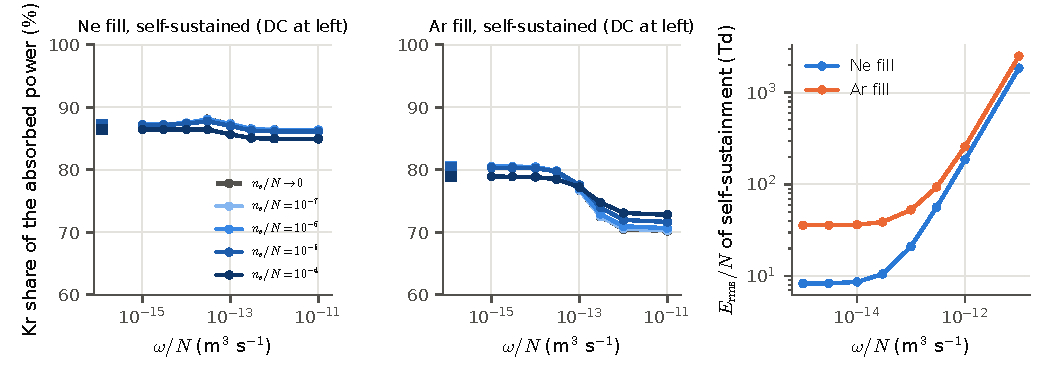
\includegraphics[width=\textwidth]{chapters/nl/fig_selfsustained.pdf}
\caption{Self-sustained discharges against $\omega/N$: krypton's share in the two
fills (DC at the left, squares) and the rms $E/N$ of self-sustainment.}
\label{nl:fig:selfsus}
\end{figure}

{\noindent}(2) In the Ne fill the discharge sustains itself at 8.33~Td DC with
87.2~\% of its power in krypton. On the grid of the scan the share peaks at
88.1~\% at $\omega/N=3\times10^{-14}$~m$^3$\,s$^{-1}$, a third of the Maxwellian
mean $\langle\nu_m\rangle/N=9.2\times10^{-14}$~m$^3$\,s$^{-1}$ at the discharge's mean
energy: the optimum sits where $\omega$ and $\nu_m$ are of the same order. A Canon
patent on microwave-excited excimer lasers states that at 35~GHz ``the plasma
excitation efficiency based on identical electric power is highest'' at the
pressure, 160~Torr, at which the collision frequency of electrons with neon, the main
body of the Kr/Ne/F$_2$ gas, equals the microwave frequency \cite{nl:Canon}. The optimum exists but is
worth 0.9 points. Far above the collision frequency the share
falls to 86.4~\%, the fatter tail exciting neon. In the Ar fill the discharge needs
35.9~Td DC and gives 80.5~\% to krypton, falling to 70.2~\% at high frequency as
argon's 11.5~eV levels take the tail. The formation efficiency moves less, from
0.351 to 0.337, because argon's excitation partly reaches KrF$^*$. Raising $n_e/N$ to
$10^{-4}$ changes these shares by at most 2.6 points.

\section{What field pumping buys}
\label{nl:sec:wallplug}

{\noindent}(1) A formation efficiency turns a
power partition into KrF$^*$ per absorbed energy,
\begin{equation}
\eta_{\rm form}=\sum_cf_c\,\frac{h\nu}{u_c}\,b_c,
\label{nl:eq:etaform}
\end{equation}
with $f_c$ the shares, $u_c$ the energy per event (Kr excitation 10.5~eV, ionization
14.0, Ne 17.5, Ar 12.5), $h\nu=4.997$~eV, and $b_c$ the branchings of a KrF kinetic
network for each fill (Kr$^*$ harpoon 0.87 and 0.81, ion channel 0.68). The same
accounting gives e-beam pumping of the Ne fill 0.175, from 30.4~eV per ion pair and 0.7
excitations per ion with this fill's Ne$^*\to$Kr$^+$ branching 0.80. That accounting
gives the beam's sub-excitation electrons
nothing. At beam-on density their e-e collisions put 0.159 of their energy into
KrF$^*$ (Sec.~\ref{nl:sec:share}, where recombination takes about a third of it), and one
such electron of 4.506~eV per 30.4~eV ion pair adds 0.024: the like-for-like e-beam
figure there is 0.198. A full kinetic model of the Ne-fill laser, whose Spencer--Fano
partition has 36.6~eV per ion pair where the chain counts 30.4, also forms 0.194 of its
deposited energy into KrF$^*$ at the photon energy, its 1.42 KrF$^*$ per ion pair
against 1.21 here making up for the larger energy per pair. The chain has no e-beam
accounting for the Ar fill.

{\noindent}(2) Field pumping of the beam-ionized gas at beam-on density has
$\eta_{\rm form}=0.327$ to 0.365 where the field dominates in the growth model
(Table~\ref{nl:tab:share}), 0.327 to 0.349 in the Ne fill, and 0.30 to 0.34 for the field's
marginal power with beam-sustained electrons in the Ne fill at 5~Td, in both attributions
and at a fixed beam current (Table~\ref{nl:tab:source} gives the fixed-$n_e$ values). The self-sustained discharge
gives 0.337 to 0.354. In the Ne fill at beam-on density, where the field's power exceeds
the beam's own, field pumping thus forms 1.5 to 1.8 times as much as the e-beam's 0.198,
and the frequency moves it by $-4$ to $+6$~\%. At 2~Td, where the beam outweighs the
field, the field's marginal power gives 0.30 to 0.33 at a fixed beam current, 1.5 to 1.7
times the e-beam's, and the frequency raises it by 9~\% (from 0.265 and by 15~\% counted
at fixed $n_e$). This is the rationale of the e-beam-controlled discharge, demonstrated for
KrF by Mangano and Jacob \cite{nl:ManganoJacob1975}, and a KrF laser pumped by the
discharge that an IR laser beam drives in the gas has also been modelled
\cite{nl:Igoshin1993}. Field pumping beats beam pumping at the wall plug when
$\eta_{\rm src}\,\eta_{\rm form,f}>\eta_{\rm beam}\,\eta_{\rm form,b}$, i.e.\ when the
source efficiency exceeds 0.57 to 0.65 of the efficiency with which the pulsed power
puts energy into the gas through the foil. The chain's branchings do not depend on
$n_e$. At beam-on density the stepwise ionization $e+{\rm Kr}^*\to{\rm Kr}^++2e$ runs at
0.39 to 1.63 of the harpoon rate in the Ne fill, rising with the power (Kannari's rate
at the scan's $T_e$ \cite{nl:Kannari1985}). It moves Kr$^*$ from the harpoon channel (0.87) to
the ion channel (0.68), which lowers the KrF$^*$ yield of a Kr$^*$ by 4.8 to 11.8~\%,
and so lowers field pumping, which goes mostly through Kr$^*$, more than beam pumping,
which goes through ions. In a full kinetic model of microwave co-pumping, the sign
of the laser energy that a co-pumping field gains rests on that one rate, and the
electron quench of KrF$^*$ is a candidate second such rate. The first
depends on $T_e$, and the second may. Those rates, not the frequency,
decide whether field pumping pays.

\section{At the target}
\label{nl:sec:ife}

{\noindent}(1) In a direct-drive corona Langdon's $\alpha_L\propto
Z_{\rm eff}I\lambda^2/T_e$ favours short wavelengths. Obenschain et al.\ computed
the quarter-critical temperature and intensity of a 2.6~mm CH sphere driven at 351,
248 and 193~nm (their Table~1, averaged over 2 to 3~ns) \cite{nl:Obenschain2020}. With
fully ionized CH, $Z_{\rm eff}=37/7$, Table~\ref{nl:tab:ife} gives $\alpha_L$ and four
estimates of $f_L$: Langdon's fit, Matte's super-Gaussian, Eq.~\eqref{nl:eq:selfsim}
with a constant logarithm, and Eq.~\eqref{nl:eq:selfsim} with the quantum logarithm
$L=\ln(2mv^2/\hbar\omega)$ of one electron in both the operator and the absorption.
The last is the kinetic counterpart of the improved factor of Turnbull et al.\
\cite{nl:Turnbull2024}, which weights a super-Gaussian with a velocity-dependent Gaunt
factor and which Sherlock et al.\ treat more thoroughly \cite{nl:Sherlock2024}. The e-e
logarithm is the NRL formulary's electron--electron value at $n_c/4$ \cite{nl:NRL},
$\lnL_{ee}=7.7$, 7.2 and 6.8 at 351, 248 and 193~nm. All of it is for a homogeneous
plasma at the time-averaged conditions, with the self-similar distribution at fixed
$\alpha_L$. Nonlocal transport near $n_c/4$ and the structure of the beam are left out.

\begin{table}[h]
\centering
\caption{The Langdon factor at the quarter-critical conditions of
\cite{nl:Obenschain2020}, Table~1. $I$ in $10^{14}$~W\,cm$^{-2}$.}
\label{nl:tab:ife}
\begin{tabular}{cccccccc}
\toprule
$\lambda$ (nm) & $T_e$ (keV) & $I$ & $\alpha_L$ & fit & Matte & kinetic, const.\ $L$ & kinetic, $L(v)$\\
\midrule
\tabinput{chapters/nl/tab_ife.tex}
\bottomrule
\end{tabular}
\end{table}

{\noindent}(2) The kinetic solution with a constant logarithm reproduces the fit
within 0.22~\%. The velocity-dependent logarithm cuts the penalty $1-f_L$ to 0.64,
0.58 and 0.52 of the fit's, in line with the finding of Turnbull et al.\ that the
velocity dependence of the Gaunt factor ``somewhat mitigates the Langdon effect''
\cite{nl:Turnbull2024}. The nonlinear factor alone makes the local absorption rate at
quarter critical higher than at 351~nm by $\times1.031$ (KrF) and $\times1.052$ (ArF)
with Langdon's fit, and by $\times1.023$ and $\times1.038$ with the velocity-dependent
logarithm. The linear coefficient itself, proportional to
$n_cT_e^{-3/2}\propto\lambda^{-2}T_e^{-3/2}$ at quarter critical apart from the
logarithm, is $\times2.53$ and $\times5.20$ that of 351~nm at the same conditions. The
nonlinearity thus adds a few percent to a much larger linear advantage of the excimer
drivers. The Langdon effect has been reviewed for laser plasmas \cite{nl:Shaffer2025},
computed for short KrF pulses on selenium \cite{nl:Pulsifer1994}, and quantified against
$I\lambda^2$ for the plasmas of extreme-ultraviolet sources, where it lowers the
absorption by 10 to 20~\% \cite{nl:GonzalezSheil2025}. No published quantification of
this wavelength dependence for excimer drivers was found, though not every candidate
could be read in full. The bandwidths of Obenschain et al.'s
Table~1, 1, 3 and 10~THz, give speckle lifetimes $1/\Delta\nu$ of 1.0, 0.33 and
0.10~ps, shorter than the e-e time $1/\nu_{ee}$ at quarter critical (4.8, 2.0 and
1.0~ps). Whether that changes the Langdon factor of a speckled beam is open. Shaffer
et al.\ found that the Langdon operator predicts the heating well in the simple cases
they considered. For a two-colour field it gave slightly less heating than their full
calculation, as it did without bandwidth, and a weaker, phase-shifted beat modulation,
which they attribute to its steady-state assumption breaking down for broadband light
\cite{nl:Shaffer2023}. The scattering of electrons on speckles changes both absorption
and transport \cite{nl:SherlockMichel2022}.

\section{Verdict and next steps}
\label{nl:sec:verdict}

{\noindent}(1) The nonlinear behavior of IB does not by itself improve a gas
laser. The lasing field of an excimer laser stays more than $10^3$ times below it. An
auxiliary field reaches only the gas nonlinearity, whose effect on the distribution the
electron--electron collisions of a pumped laser largely supply: what is left of the
frequency's advantage at the beam-on density is 2 to 7~\% where the field's power
exceeds the beam's own and 10 to 14~\% at a fixed beam current where the beam's is larger
(1 to 18~\% without recombination), and up to $\times1.24$ at a fixed beam current
($\times1.355$ at fixed $n_e$) at the five times lower density that this note's electron
source and losses give with the beam of the full kinetic model. At the target the
nonlinearity
is worth a few percent of absorption rate to KrF and ArF. The ranked next steps,
cheapest decisive first:
\begin{enumerate}
\item \emph{The instrument.} Fit THz transmission of the laser gas with this
  solver, which carries the field, the ions and e-e, to read $n_e$ and $T_e$, and
  use a THz $T_e$ jump to measure $e+{\rm Kr}^*\to{\rm Kr}^++2e$ and the electron
  quench of KrF$^*$. The first decides the sign of the
  co-pump in a full kinetic model, the second is the candidate for a second such rate.
\item \emph{Field co-pumping at beam-class power}, frequency-blind: run a full kinetic
  model of the laser in pairs, with and without the field, with this solver's partition
  (Tables~\ref{nl:tab:share} and~\ref{nl:tab:source}) and the uncertain rates bracketed, with the
  electron collisions on Kr$^*$ and KrF$^*$ that the formation chain leaves out.
\item \emph{The e-beam's own sub-excitation electrons.} Item~(3) of
  Sec.~\ref{nl:sec:share} sends 39~\% of their energy to krypton at beam-on density
  through e-e collisions in the Ne fill (45~\% in the Ar fill), which raises the
  e-beam's formation efficiency from 0.175 to 0.198. Check whether the energy
  accounting of full kinetic models of the laser carries it.
\item \emph{The electron source.} The residual advantage at beam-on density depends
  on how the electrons are created and lost and on how the field's share is counted
  (1 to 28~\%), and on the density itself, which this note's electron source and losses
  and a full kinetic model put about five times apart. Held at a fixed beam current in the steady state it is within 0.01
  of the fixed-beam ratio (Sec.~\ref{nl:sec:source}). A run in time with the beam's source,
  attachment, recombination on the fill's own mix of cations and the field together
  would settle it.
\item \emph{CO$_2$ lasers.} Of the lasers examined, the one whose own field heats
  its electrons at the 10~\% level, by an order-of-magnitude estimate. Compute it with
  the discharge's own distribution and timing, and its effect on the vibrational
  partition and on discharge stability for high-intensity amplifiers.
\item \emph{The target.} Use the velocity-dependent Langdon factor in the
  wavelength studies of excimer drivers, and test whether THz bandwidth and speckle
  change it.
\end{enumerate}

\chapterappendix
\section{The electron--electron operator in energy}
\label{nl:app:ee}

{\noindent}(1) The isotropic Rosenbluth operator for electrons of distribution
$f(v)$, $\int4\pi v^2f\,\dd v=n_e$, is \cite{nl:Rosenbluth1957}
\begin{equation}
\frac{\partial f}{\partial t}=\frac{4\pi\Gamma}{v^2}\frac{\partial}{\partial v}
\Big[f\,I_2+\frac{I_4+v^3J_1}{3v}\frac{\partial f}{\partial v}\Big],\qquad
\Gamma=\frac{e^4\lnL}{4\pi\epsilon_0^2m^2},
\end{equation}
with $I_2=\int_0^vu^2f$, $I_4=\int_0^vu^4f$, $J_1=\int_v^\infty uf$. For a
Maxwellian $J_1=v_t^2f$ and $I_4=3v_t^2I_2-v^3v_t^2f$, so the bracket vanishes.

{\noindent}(2) Write $h(v,w)=\min(v,w)^3/3$. Since $\partial_wh=w^2$ for $w<v$
and 0 above, $-\int f'(w)h\,\dd w=I_2$. And $(I_4+v^3J_1)/3v=\int f(w)(w/v)h\,\dd w$.
The bracket is therefore
\begin{equation}
\int_0^\infty w\,h(v,w)\Big[f(w)\frac{f'(v)}{v}-f(v)\frac{f'(w)}{w}\Big]\dd w,
\end{equation}
so $v$ times the bracket has the symmetric weight $v\,w\,h$ and an antisymmetric
bracket, which is the Landau form. In energy, $f'(v)/v=(m/e)\,\partial_\epsilon f$ and
$w\,\dd w=(e/m)\dd\epsilon'$, and with $f=n_e(2\pi)^{-1}(m/2e)^{3/2}F$ the upward
number flux per electron becomes Eq.~\eqref{nl:eq:ee-landau}.

{\noindent}(3) Integrating by parts in $\epsilon'$,
$\int\min^{3/2}[F(\epsilon')F'-FF'(\epsilon')]\dd\epsilon'=F'(A_2+\epsilon^{3/2}A_3)+\tfrac32A_1F$,
which is half the bracket of Hagelaar and Pitchford, so their $a$ \cite{nl:HP2005}
equals $(2\Gamma/3)(m/2e)^{3/2}=e^2\gamma\lnL/24\pi\epsilon_0^2$, as written in
Eq.~\eqref{nl:eq:ee-landau}.

\section{The checks}
\label{nl:app:checks}

\noindent A check script computes every result, or reloads it from the stored output
of the scan that made it and recomputes a sample of that output, and tests it. It
recomputes the computed numbers of the prose to their printed digits, each inside a
sentence that occurs once in the text, compares the inputs the text states with the
code that uses them, and tests the worded claims against the data. It re-derives the
displayed formulas numerically and requires them in the text as printed. The numbers
quoted from sources were checked against the sources by hand. Table~\ref{nl:tab:checks}
counts the checks by the section they support.

{\small
\begin{longtable}{L{6.4cm}ccc}
\caption{The checks of these notes, by the section whose statements, equations, tables and figures they support: all checks, the computed numbers of the prose recomputed to their printed digits, and the worded claims tested against the data.}\label{nl:tab:checks}\\
\toprule
supports & checks & printed numbers & claims\\
\midrule
\endfirsthead
\toprule
supports & checks & printed numbers & claims\\
\midrule
\endhead
\bottomrule
\endfoot
Sec.~\ref*{nl:sec:answer} & 58 & 40 & 16\\
Sec.~\ref*{nl:sec:three} & 18 & 8 & 1\\
Sec.~\ref*{nl:sec:kinetic} & 46 & 12 & 5\\
Sec.~\ref*{nl:sec:checks} & 20 & 8 & 3\\
Sec.~\ref*{nl:sec:regime} & 45 & 20 & 19\\
Sec.~\ref*{nl:sec:share} & 150 & 95 & 30\\
Sec.~\ref*{nl:sec:selfsus} & 23 & 14 & 5\\
Sec.~\ref*{nl:sec:wallplug} & 61 & 47 & 4\\
Sec.~\ref*{nl:sec:ife} & 29 & 18 & 4\\
Sec.~\ref*{nl:sec:verdict} & 17 & 14 & 3\\
Appendix~\ref*{nl:app:ee} & 1 &  & \\
Appendix~\ref*{nl:app:checks} & 2 &  & \\
the references and the text as a whole & 65 &  & \\
\midrule
Total & 535 & 276 & 90\\
\end{longtable}
}


\raggedright
\begin{thebibliography}{99}
\bibitem{nl:Langdon1980} A. B. Langdon, Nonlinear inverse bremsstrahlung and
heated-electron distributions, Phys. Rev. Lett. \textbf{44}, 575 (1980),
doi:10.1103/PhysRevLett.44.575.
\bibitem{nl:Matte1988} J. P. Matte, M. Lamoureux, C. M\"oller, R. Y. Yin,
J. Delettrez, J. Virmont and T. W. Johnston, Non-Maxwellian electron
distributions and continuum X-ray emission in inverse bremsstrahlung heated
plasmas, Plasma Phys. Control. Fusion \textbf{30}, 1665 (1988),
doi:10.1088/0741-3335/30/12/004.
\bibitem{nl:Turnbull2023} D. Turnbull et al., Inverse bremsstrahlung absorption,
Phys. Rev. Lett. \textbf{130}, 145103 (2023), doi:10.1103/PhysRevLett.130.145103.
\bibitem{nl:Turnbull2024} D. Turnbull et al., Reconciling calculations and
measurements of inverse bremsstrahlung absorption, Phys. Plasmas \textbf{31},
063304 (2024), doi:10.1063/5.0203446.
\bibitem{nl:Milder2021} A. L. Milder et al., Measurements of non-Maxwellian electron
distribution functions and their effect on laser heating, Phys. Rev. Lett.
\textbf{127}, 015001 (2021), doi:10.1103/PhysRevLett.127.015001.
\bibitem{nl:QBE} C. K. Watson et al., Unified microscopic foundations of the quantum
Boltzmann equation, Fluct. Noise Lett. \textbf{25}, 2640002 (2026),
doi:10.1142/S021947752640002X.
\bibitem{nl:Atzeni2004} S. Atzeni and J. Meyer-ter-Vehn, \emph{The Physics of Inertial
Fusion} (Oxford University Press, Oxford, 2004),
doi:10.1093/acprof:oso/9780198562641.001.0001.
\bibitem{nl:Glyavin2012} M. Yu. Glyavin, A. G. Luchinin, G. S. Nusinovich, J. Rodgers,
D. G. Kashyn, C. A. Romero-Talamas and R. Pu, A 670 GHz gyrotron with record power and
efficiency, Appl. Phys. Lett. \textbf{101}, 153503 (2012), doi:10.1063/1.4757290.
\bibitem{nl:HP2005} G. J. M. Hagelaar and L. C. Pitchford, Solving the Boltzmann
equation to obtain electron transport coefficients and rate coefficients for fluid
models, Plasma Sources Sci. Technol. \textbf{14}, 722 (2005),
doi:10.1088/0963-0252/14/4/011.
\bibitem{nl:Rosenbluth1957} M. N. Rosenbluth, W. M. MacDonald and D. L. Judd,
Fokker--Planck equation for an inverse-square force, Phys. Rev. \textbf{107}, 1
(1957), doi:10.1103/PhysRev.107.1.
\bibitem{nl:WalkerNi2011} H. F. Walker and P. Ni, Anderson acceleration for
fixed-point iterations, SIAM J. Numer. Anal. \textbf{49}, 1715 (2011),
doi:10.1137/10078356X.
\bibitem{nl:Druyvesteyn1940} M. J. Druyvesteyn and F. M. Penning, The mechanism of
electrical discharges in gases of low pressure, Rev. Mod. Phys. \textbf{12}, 87
(1940), doi:10.1103/RevModPhys.12.87.
\bibitem{nl:Margenau1946} H. Margenau, Conduction and dispersion of ionized gases at
high frequencies, Phys. Rev. \textbf{69}, 508 (1946), doi:10.1103/PhysRev.69.508.
\bibitem{nl:Obenschain2020} S. P. Obenschain et al., Direct drive with the argon
fluoride laser as a path to high fusion gain with sub-megajoule laser energy,
Phil. Trans. R. Soc. A \textbf{378}, 20200031 (2020), doi:10.1098/rsta.2020.0031.
\bibitem{nl:Canon} T. Ohmi, N. Tanaka and M. Hirayama (Canon Inc.), Excimer laser
oscillation apparatus and method, excimer laser exposure apparatus, and laser tube,
US Patent 6,331,994 B1 (published 2001-12-18).
\bibitem{nl:Silin1965} V. P. Silin, Nonlinear high-frequency plasma conductivity,
Sov. Phys. JETP \textbf{20}, 1510 (1965) [Zh. Eksp. Teor. Fiz. \textbf{47}, 2254
(1964)], record at \url{http://www.jetp.ras.ru/cgi-bin/e/index/e/20/6/p1510?a=list}.
\bibitem{nl:Karoulina1988} E. V. Karoulina and Yu. A. Lebedev, The influence of the
electron transport cross sectional shape on electron energy distribution functions in
DC and microwave plasmas, J. Phys. D \textbf{21}, 411 (1988),
doi:10.1088/0022-3727/21/3/006.
\bibitem{nl:FerreiraLoureiro1983} C. M. Ferreira and J. Loureiro, Electron energy
distributions and excitation rates in high-frequency argon discharges, J. Phys. D
\textbf{16}, 2471 (1983), doi:10.1088/0022-3727/16/12/024.
\bibitem{nl:Sa1992} P. A. S\'a, J. Loureiro and C. M. Ferreira, Effects of
electron--electron collisions on the characteristics of DC and microwave discharges
in argon at low pressures, J. Phys. D \textbf{25}, 960 (1992),
doi:10.1088/0022-3727/25/6/010.
\bibitem{nl:Wang1993} D. Wang, T. Ma and B. Guo, Electron energy distributions and
kinetic temperatures in high-frequency argon discharges, J. Phys. D \textbf{26}, 62
(1993), doi:10.1088/0022-3727/26/1/010.
\bibitem{nl:Igoshin1993} V. I. Igoshin and S. Yu. Pichugin, Pumping a KrF excimer laser
by a laser discharge induced by an IR laser beam, Quantum Electron. \textbf{23}, 33
(1993), doi:10.1070/QE1993v023n01ABEH002931.
\bibitem{nl:Shaffer2025} N. R. Shaffer, T. Seo, S. X. Hu and V. N. Goncharov, The
Langdon effect in laser plasmas: Absorption and conduction, Phys. Plasmas
\textbf{32}, 062703 (2025), doi:10.1063/5.0266182.
\bibitem{nl:Pulsifer1994} P. E. Pulsifer and K. G. Whitney, Fokker--Planck analysis of
short-pulse laser heating in the hot-spot-model approximation, Phys. Rev. E
\textbf{50}, 4926 (1994), doi:10.1103/PhysRevE.50.4926.
\bibitem{nl:Shaffer2023} N. R. Shaffer, M. Sherlock, A. V. Maximov and V. N. Goncharov,
An extended Vlasov--Fokker--Planck approach for kinetic simulations of laser plasmas,
Phys. Plasmas \textbf{30}, 043906 (2023), doi:10.1063/5.0143248.
\bibitem{nl:SherlockMichel2022} M. Sherlock and P. Michel, Absorption and transport
effects induced in plasmas by the interaction of electrons with laser speckles,
Phys. Rev. Lett. \textbf{129}, 215001 (2022), doi:10.1103/PhysRevLett.129.215001.
\bibitem{nl:Tachikawa1990} M. Tachikawa, H. Murakami, F. O. Shimizu and T. Shimizu, Novel
aspects of the optogalvanic effect in the CO$_2$ laser medium, Jpn. J. Appl. Phys.
\textbf{29}, 958 (1990), doi:10.1143/JJAP.29.958.
\bibitem{nl:LXCat} E. Carbone et al., Data needs for modeling low-temperature
non-equilibrium plasmas: the LXCat project, history, perspectives and a tutorial, Atoms
\textbf{9}, 16 (2021), doi:10.3390/atoms9010016; the BSR, Biagi-v7.1, IST-Lisbon and
SIGLO databases at www.lxcat.net.
\bibitem{nl:NRL} A. S. Richardson, \emph{2019 NRL Plasma Formulary} (Naval Research
Laboratory, Washington, DC, 2019).
\bibitem{nl:GinzburgGurevich1960} V. L. Ginzburg and A. V. Gurevich, Nonlinear phenomena
in a plasma located in an alternating electromagnetic field, Sov. Phys. Usp.
\textbf{3}, 115 and 175 (1960), doi:10.1070/PU1960v003n01ABEH003261 and
doi:10.1070/PU1960v003n02ABEH003267.
\bibitem{nl:Gurevich1978} A. V. Gurevich, \emph{Nonlinear Phenomena in the Ionosphere}
(Springer, Berlin, 1978), doi:10.1007/978-3-642-87649-3.
\bibitem{nl:Kannari1985} F. Kannari, M. Obara and T. Fujioka, An advanced kinetic model of
electron-beam-excited KrF lasers including the vibrational relaxation in KrF$^*$(B) and
collisional mixing of KrF$^*$(B,C), J. Appl. Phys. \textbf{57}, 4309 (1985),
doi:10.1063/1.334590.
\bibitem{nl:Sakamoto2007} K. Sakamoto et al., Achievement of robust high-efficiency 1~MW
oscillation in the hard-self-excitation region by a 170~GHz continuous-wave gyrotron,
Nature Phys. \textbf{3}, 411 (2007), doi:10.1038/nphys599.
\bibitem{nl:ManganoJacob1975} J. A. Mangano and J. H. Jacob, Electron-beam-controlled
discharge pumping of the KrF laser, Appl. Phys. Lett. \textbf{27}, 495 (1975),
doi:10.1063/1.88547.
\bibitem{nl:Sherlock2024} M. Sherlock, P. Michel, D. J. Strozzi, L. Divol, E. Kur and
G. Zimmerman, Inverse bremsstrahlung absorption rate for super-Gaussian electron
distribution functions including plasma screening, Phys. Rev. E \textbf{109}, 055201
(2024), doi:10.1103/PhysRevE.109.055201.
\bibitem{nl:GonzalezSheil2025} J. Gonzalez and J. Sheil, Langdon effect in the realm of
extreme ultraviolet source plasmas, Phys. Rev. E \textbf{111}, L023201 (2025),
doi:10.1103/PhysRevE.111.L023201.
\end{thebibliography}
\endgroup
